% Chapter Template

\chapter{Jets and PU at stage 2} % Main chapter title

\label{Chapter 7} % Change X to a consecutive number; for referencing this chapter elsewhere, use \ref{ChapterX}

\lhead{Chapter 7. \emph{Conclusions}} % Change X to a consecutive number; this is for the header on each page - perhaps a shortened title

%----------------------------------------------------------------------------------------
%	SECTION 1
%----------------------------------------------------------------------------------------

\section{Jet Algorithm}
\label{algo}
The focus of the results in this report will be on studies for jet definitions and pile-up subtraction algorithms for the stage 2 trigger. At stage 2 the TMT allows the granularity to be significantly increased compared to the legacy system. The cells used to make the jets will reduce from $4\times4$ towers to single towers. Due to the increase in energy to 13TeV the jets will be boosted and therefore smaller in size. To account for this at level one the cone size should be decreased. The algorithm presented here uses a cone size of 9 by 9 compared to 12 by 12 which corresponds to the decrease from R=0.5 to R=0.4 in the jet definition proposed for HLT (CITE??). Jets from the primary vertex are likely to be boosted and thus most of their energy is in the central (seed) tower. The algorithm is thus as follows: each trigger tower in turn is taken as the candidate. The towers in the 4 surrounding rings (or up to the edge in $\eta$) are then compared to the seed tower using the mask shown in figure \ref{mask}. If the comparison is true for any tower then the seed is vetoed and the next tower is checked. The mask is designed to be unambiguous for towers of equal energy. If a seed is not vetoed then a jet is defined at that tower position with $p_t$ given by the total energy of the towers.   
\begin{figure}
\centering
    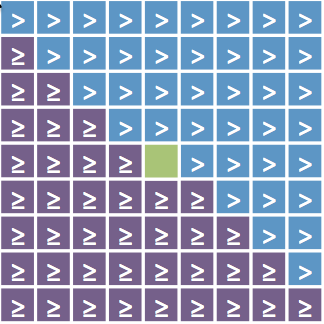
\includegraphics[width=0.5\textwidth]{Figures/mask.png}
  \caption{Nine by nine mask used to define jets}
  \label{mask}
\end{figure}
\newpage
The two main problems with this algorithm are that sufficiently close jets will appear as a single jet and that energy may be lost if a tower that vetoes another is itself vetoed by a tower sufficiently far away not to include the far tower's energy. The first case is common to all jet algorithms with a fixed cone size but as the energy is not lost the single jet or total energy will almost certainly be enough to trigger. Despite this a quality bit adapted from the idea of n-subjetiness \cite{nsub} is under investigation. The lost energy is found to be a small (~0.1\% inefficiency).
%%///ASKJAD%%%
\section{Jet Algorithm}
The focus of the results in this report will be on studies for jet definitions and pile-up subtraction algorithms for the stage 2 trigger. At stage 2 the TMT allows the granularity to be significantly increased compared to the legacy system. The cells used to make the jets will reduce from $4\times4$ towers to single towers. Due to the increase in energy to 13TeV the jets will be boosted and therefore smaller in size. To account for this at level one the cone size should be decreased. The algorithm presented here uses a cone size of 9 by 9 compared to 12 by 12 which corresponds to the decrease from R=0.5 to R=0.4 in the jet definition proposed for HLT (CITE??). Jets from the primary vertex are likely to be boosted and thus most of their energy is in the central (seed) tower. The algorithm is thus as follows: each trigger tower in turn is taken as the candidate. The towers in the 4 surrounding rings (or up to the edge in $\eta$) are then compared to the seed tower using the mask shown in figure \ref{mask}. If the comparison is true for any tower then the seed is vetoed and the next tower is checked. The mask is designed to be unambiguous for highest towers of equal energy. If the seed is not vetoed then a jet is defined at that tower position with $p_t$ given by the total energy of the towers.    
\begin{figure}
\centering
    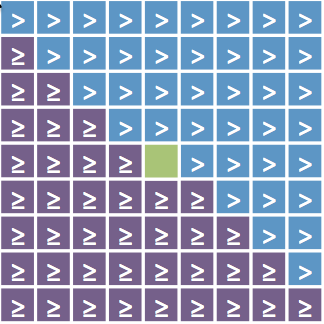
\includegraphics[width=0.5\textwidth]{Figures/mask.png}
  \caption{Nine by nine mask used to define jets}
  \label{mask}
\end{figure}
\newpage
The two main problems with this algorithm are that sufficiently close jets will appear as a single jet and that energy may be lost if a tower that vetoes another is itself vetoed by a tower sufficiently far away not to include the far tower's energy. The first case is common to all jet algorithms with a fixed cone size to avoid duplication of energy but as the energy is not lost the single jet or total energy will almost certainly be enough to trigger. Despite this, a quality bit adapted from the idea of n-subjetiness \cite{nsub} is under investigation this would allow a jet with substructure but with lower energy than the single jet threshold to trigger. The energy lost by a 'chain' veto is an unavoidable inefficiency, however, the effect of this is seen to be small in the matching (~0.1\% inefficiency) (see figure**).

\section{Pile Up Subtraction}
\subsection{Pile Up}
The luminosity of the LHC will be increased in the upgrade to $L = 1\times10^{34} cm^{-2}s^{-1}$. The easiest way to increase luminosity while maintaining stability is to use large, but widely separated, proton bunches \cite{pileup}. However, for the detector this means increased number of primary vertices (pile up) at the collision point. The average number of vertices per bunch crossing is given in equation \ref{pu}.

\begin{equation}
\langle N_p \rangle = \sigma L \tau_b
\label{pu}
\end{equation}

where $\langle N_p \rangle$ is the average number of vertices, $\sigma$ is the cross section and $\tau_b$ is the bunch spacing. At the end of run 1 with $8 TeV$ ($\sigma = 71.5mb$),$\tau_b = 50ns$ and $L = 0.75\times10^{34} cm^{-2}s^{-1}$ gave $\langle N_p \rangle$ = 27. After LS1 the luminosity and $\sigma$ gain (to $76mb$) this will increase to $\langle N_p \rangle$ = 40. 
\subsection{Effect of Pile Up}
The majority of PU events are low energy QCD processes which will appear as randomly distributed energy in the calorimeter region (about 1 GeV per unit area). This PU can have two detrimental effects for the L1 trigger. Firstly, when the PU is evenly distributing the energy of the real jets is slightly increased thus artificially increasing the total transverse energy. The second problem occurs when the PU is randomly clustered - significantly boosting a single jet or forming fake jets. Due to the non perfect response of the detector and profile of the PU these effects may be dependent on $\eta$. In order to trigger only on hard events the effect of the PU must be mitigated (subtracted). In this report two example methods of pileup subtraction (global $\rho$ and donut) will be discussed.
\subsection{Subtraction}

M. Cacciari and G. P. Salam, “Pileup subtraction using jet areas,” Phys.Lett., vol. B659, pp. 119–126, 2008

If the detector response is assumed to be approximately $\eta$ independent then one may use an event based PU subtraction. In the case of global $\rho$ first all the jets are reconstructed using the algorithm in \ref{algo}. The jets are then ranked in order of energy density $\rho$ where for jet i, $\rho^i$ is defined in equation \ref{rho}.
\begin{equation}
\label{rho}
\rho^i = \frac{p^i_{T}}{A_i} 
\end{equation}
where $A_i$ is the area of the jet. The median $\rho$ ($\rho^m$) of the jets is then taken as the estimator of the PU energy density in the event. All jets are in the event then reduced in energy by $\rho^m \times A^i$ and those with $p_{T}^i < \rho^m \times A_i$ taken to be PU and removed. The correlation of this parameter with the number of vertices is shown in figure **. This method has the advantage of being stable against fluctuations however local effects are not considered and there is inherent under-subtraction bias as the PU jet $p_{T}$ forms a bound on the energy subtracted per jet.

Donut subtraction takes advantage of the area around each jet to make a local subtraction. Taking the four strips around the jet as shown in figure ** they are ordered in energy and the pile up energy density is taken as the energy of the middle strips divided by their area ($A_d$).      
